\section{Forecasts}

\subsection{Optimising Design Variables}

There is only so much funding one can get to carry out science. In order to get the best return on time and money invested, you want to know what you're studying and how best to measure it. This is no different for PMF detection. In order to find the best experimental set up and

In order to find the best experimental set up and quantify the improvement from stage-2 to stage-3 or stage-4, I used the mock covariances as described in section 3.3. By varying one experimental variable at a time and holding the rest fixed, I was able to forecast the minimum uncertainty on the PMF strength, $\sigma(B_{1Mpc})$ for each mock experiment and plot the relationship between $\sigma(B_{1Mpc})$ and the experimental variables.

\begin{figure}[h]
\centering
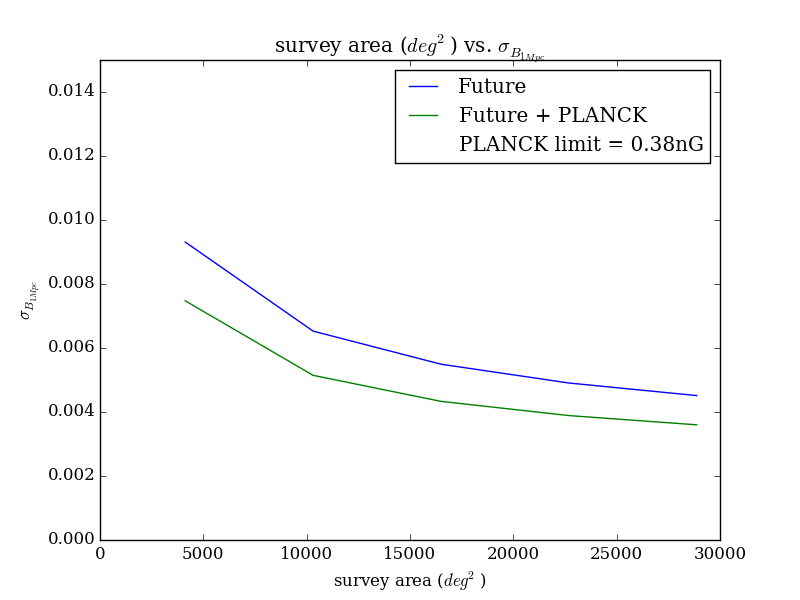
\includegraphics[scale=0.8]{images/area.png}
\caption{Plot of survey area vs the experimental uncertainty on $B_{1Mpc}$ with all other independent experimental variables held fixed. This plot shows that as the survey area of an experiment increases, the precision on $B_{1Mpc}$ improves, thus the ideal experiment for detecting PMFs will increase the survey area. The blue line shows the precision for Future CMB experiments on their own and the green line shows the same precisions when combined with the PLANCK data set. The data shows a drastic improvement over previous PLANCK constraints of $\sigma(B_{1Mpc}) \geq 0.38nG$.}
\label{fig:area}
\end{figure}

\begin{figure}[h]
\centering
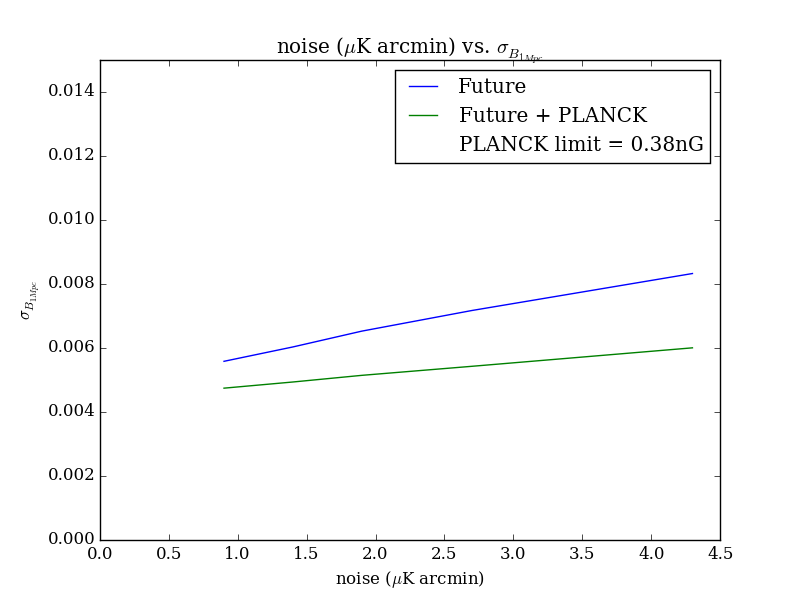
\includegraphics[scale=0.8]{images/noise.png}
\caption{Plot of noise vs the predicted experimental uncertainty on $B_{1Mpc}$. This plot shows that, as expected, reducing the nosie levels (adding more detectors) improves the constraints on $B_{1Mpc}$. The blue line shows the predicted limits on $\sigma(B_{1Mpc})$ from future CMB experiments and the green line shows the predicted limits on $\sigma(B_{1Mpc})$ for future experiments combined with current PLANCK constraints. The data shows a significant increase in precision over PLANCK's constraints alone, which were $\sigma(B_{1Mpc}) \geq 0.38nG$.}
\label{fig:noise}
\end{figure}

\begin{figure}[h]
\centering
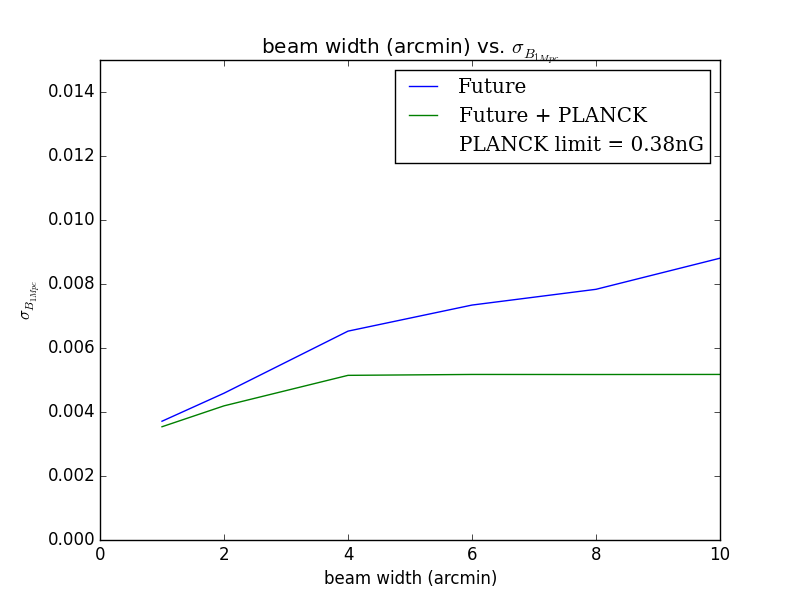
\includegraphics[scale=0.8]{images/width.png}
\caption{Plot of beam width vs the experimental uncertainty on $B_{1Mpc}$. This plot shows that reducing the width of the beam reduces the uncertainty on $B_{1Mpc}$. The blue line shows the best constraints for $B_{1Mpc}$ for future CMB experiments and the green like shows the best constraints for $B_{1Mpc}$ for future CMB experiments plus PLANCK's constraints. Future experiments are expected to improve upon PLANCK's limit of $\sigma(B_{1Mpc}) \geq 0.38nG$ by a wide margin.}
\label{fig:width}
\end{figure}

\begin{figure}[h]
\centering
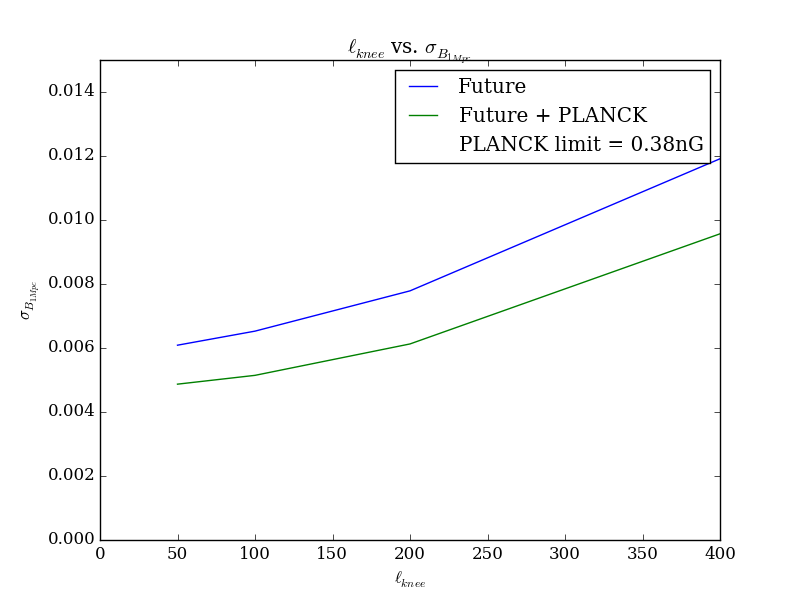
\includegraphics[scale=0.8]{images/knee.png}
\caption{Plot of $\ell_{knee}$ vs experimental uncertainty on $B_{1Mpc}$ with all other variables held fixed. This plot shows that precision on $B_{1Mpc}$ decreases as $\ell_{knee}$ increases, so it is best to reduce $\ell_{knee}$. The blue line shows the best possible $\sigma(B_{1Mpc})$ for future experiments and the green line shows the best constraints for $\sigma(B_{1Mpc})$ for future experiments combined with prior limits from PLANCK. The data shows vast improvements over PLANCK's previous limit of $\sigma(B_{1Mpc}) \geq 0.38nG$}
\label{fig:knee}
\end{figure}
\pagebreak

While varying the experimental design, the fixed values need to be chosen with care. The choice of values will determine how reliable the following forecasts are. The values I chose for the variables are more characteristic to stage-3 experiments than stage-4 ones. The average survey area of a stage-3 experiment is of the order $\sim$10 000 square degrees (roughly one quarter of the sky). On the other hand, stage-4 experiments are expected to achieve approximately half-sky coverage. Since I chose the stage-3 expected sky coverage, we can expect that the forecasts will underestimate the accuracy gains for stage-4 experiments. On the whole, the values I chose reflect the design specifications of a stage-3 experiment so we would expect the forecasts for stage-4 improvements to be conservative. Table ~\ref{table: fixed-stats} shows the values chosen for a variable when it was held fixed.

\begin{table}[h]
\centering
\caption{Fixed Variables}

\label{table: fixed-stats}
\begin{tabular}{l|l}
\multicolumn{1}{c}{Variable} & \multicolumn{1}{|c}{Value} \\ \hline
\multicolumn{1}{c}{Survey area $(deg^2)$} & \multicolumn{1}{|c}{10313}  \\
\multicolumn{1}{c}{Noise ($\mu$K arcmin)} & \multicolumn{1}{|c}{1.9}   \\
\multicolumn{1}{c}{$\ell_{knee}$} & \multicolumn{1}{|c}{100} \\
\multicolumn{1}{c}{beam width (arcmin)} & \multicolumn{1}{|c}{4.0}   \\
\multicolumn{1}{c}{calibration error (\% error)} & \multicolumn{1}{|c}{0.01} \\
\multicolumn{1}{c}{beam uncertainty (\% error)} & \multicolumn{1}{|c}{0.05}
\end{tabular}
\begin{flushleft}
This table shows the values I chose for each independent variable when they were held fixed. The variables shown are all generous estimates for the range of capabilities the stage-3 experiments will have, but very conservative for stage-4. As a result, the forecasts will underestimate the strengths for the best-case scenario stage-4 experiments.
\end{flushleft}
\end{table}

The forecasts for the next stages of CMB experiments are promising. Our current best limits from Planck are $\sigma(B_{1Mpc}) \geq 0.38nG$. In comparison, the limits from stage-3 and stage-4-like covariances fall within the range of $\sim$ 0.01nG to $\sim$ 0.001nG. In the most optimistic cases, measurements will have 100 times more sensitivity to PMFs than current experiments.

The optimal experimental design for detecting PMFs maximises the survey area and minimises the beam width, noise and $\ell_{knee}$. The sensitivity is independent of the beam and calibration uncertainties. 

As shown in figure ~\ref{fig:area}, $\sigma(B_{1Mpc})$ decreases as the survey area increases. If we combine the mock covariances with PLANCK data our best constraints range from $\sigma(B_{1Mpc}) \geq 0.0075nG$ for a survey area of 4125 deg$^2$ to $\sigma(B_{1Mpc}) \geq 0.0036nG$ for a survey area of 28877 deg$^2$, improving by a factor of 2.08. We also see a factor of 1.28 improvement, when the noise decreases from 4.3 $\mu$K arcmin to 0.9 $\mu$K arcmin, yielding  $\sigma(B_{1Mpc}) \geq 0.0060nG$ and $\sigma(B_{1Mpc}) \geq 0.0048nG$ respectively, as seen in figure ~\ref{fig:noise}. Decreasing the beam width from 10 arcmin to 1 arcmin improves sensitivity by a factor of 1.46 by reducing the uncertainty from $\sigma(B_{1Mpc}) \geq 0.0052nG$ to $\sigma(B_{1Mpc}) \geq 0.0035nG$ as per figure ~\ref{fig:width}. In figure ~\ref{fig:knee}, we see that a lower $\ell_{knee}$ improves sensitivity. At $\ell_{knee} = 50$, $\sigma(B_{1Mpc}) \geq 0.0049nG$ and in the worst-case scenario, when $\ell_{knee} = 400$, we have $\sigma(B_{1Mpc}) \geq 0.0096nG$ - a factor of 1.96 improvement. In contrast, changes to calibration and beam uncertainty have negligible effects on improving detection limits. For all values of beam and calibration uncertainties the sensitivity to the PMF strength is $\sigma(B_{1Mpc}) \geq 0.0051nG$.

\pagebreak
\subsection{Parameter Constraints}

Constraining the field strength of PMFs is not the only science goal of future CMB experiments. These experiments are also expected to constrain a wide variety of other model parameters characteristic of extensions to $\Lambda CDM$ cosmology. In this section I will provide the 1$\sigma$ confidence contours for $B_{1Mpc}$ and the selection of extended model parameters as described in Section 3.

By inverting Fisher matrices into covariance matrices, one can construct confidence ellipses for pairs of model parameters. The major and minor axes of the ellipse, $R_{major}$ and $R_{minor}$ are given by:

\begin{equation}
R_{major} = \sqrt{\frac{(\sigma_{xx} + \sigma_{yy})}{2} + \sqrt{\frac{(\sigma_{xx} - \sigma_{yy})^2}{4} + \sigma_{xy}^2}}
\end{equation}

\begin{equation}
R_{minor} = \sqrt{\frac{(\sigma_{xx} + \sigma_{yy})}{2} - \sqrt{\frac{(\sigma_{xx} - \sigma_{yy})^2}{4} + \sigma_{xy}^2}}
\end{equation}

where $\sigma{xy}$ are the covariances for the $x^{th}$ and $y^{th}$ model parameter. The angle of orientation of the confidence ellipse, $\theta$ is given by:

\begin{equation}
\theta = \frac{1}{2}arctan(\frac{2\sigma_{xy}}{\sigma_{xx}-\sigma_{yy}})
\end{equation}

For each contour plot, there are 3 ellipses. The red ellipse represents the present day constraints on the extended model parameters from PLANCK. The blue ellipse represents the forecasted constraints from a typical stage-3 CMB experiment plus PLANCK data. The green ellipse represents the forecasted constraints from a typical stage-4 CMB experiment plus PLANCK data. For this analysis I set the typical stage-3 experiment as having a survey area of 10313 square degrees, a noise level of 2.7$\mu$K arcmin and $\ell_{knee} = 100$. The typical stage-4 experiment improves on these variables with approximately two times the survey area, 22689 square degrees, half the noise, at 1.3$\mu$K arcmin and $\ell_{knee} = 50$. Table ~\ref{table: stage-stats} shows the full set of 'typical' values I chose for the experimental variables of stage-3 and stage-4 experiments.

\begin{table}[h]
\centering
\caption{Mock Stage-3 and Stage-4 Variables}

\label{table: stage-stats}
\begin{tabular}{l|l|l}
\multicolumn{1}{c}{Variable} & \multicolumn{1}{|c}{Stage-3} & \multicolumn{1}{|c}{Stage-4} \\ \hline
\multicolumn{1}{c}{Survey area $(deg^2)$} & \multicolumn{1}{|c}{10313} & \multicolumn{1}{|c}{22689}  \\
\multicolumn{1}{c}{Noise ($\mu$K arcmin)} & \multicolumn{1}{|c}{2.7} & \multicolumn{1}{|c}{1.3}  \\
\multicolumn{1}{c}{$\ell_{knee}$} & \multicolumn{1}{|c}{100} & \multicolumn{1}{|c}{50} \\
\multicolumn{1}{c}{beam width (arcmin)} & \multicolumn{1}{|c}{4.0} & \multicolumn{1}{|c}{4.0}   \\
\multicolumn{1}{c}{calibration error (\% error)} & \multicolumn{1}{|c}{0.01} & \multicolumn{1}{|c}{0.01} \\
\multicolumn{1}{c}{beam uncertainty (\% error)} & \multicolumn{1}{|c}{0.05} & \multicolumn{1}{|c}{0.05}
\end{tabular}
\\
\begin{flushleft}
This table shows the values for each variable for both the mock covariance matrices used to construct the confidence ellipses. We see that from stage-3 to stage-4, the survey area will more than double from 10313 square degrees to 22689 square degrees, the noise will halve from 2.7$\mu$K arcmin to 1.3$\mu$K arcmin as will $\ell_{knee}$ - from 100 to 50. On the other hand, beam width will remains fixed at 4.0 arcmin and both beam and calibration errors stay at 0.05$\%$ and 0.01$\%$ respectively.
\end{flushleft}
\end{table}

As shown in figure ~\ref{fig:nrun}, stage-3 and stage-4 experiments make major improvements on $B_{1Mpc}$ and moderate improvements over $n_{run}$ from PLANCK results. The gains in precision in $n_{run}$ are significant from stage-3 to stage-4 in contrast to the gains in $B_{1Mpc}$. This relationship between $\sigma({B_{1Mpc})$ and $\sigma({n_{run})$ indicates that future CMB experiments will be effective for providing constraints on $n_{run}$. Additionally, There is a very weak degeneracy between the two parameters according to the PLANCK contour which seems to be broken by the contours from stage-3 and stage-4.

Figure ~\ref{fig:neff} shows that stage-3 and stage-4 experiments make moderate improvements on constraining $N_{eff}$ from current PLANCK results. The graph also shows that within PLANCK data there exists a degeneracy between the $B_{1Mpc}$ and the effective number of neutrinos. Stage-3 and stage-4 appear to break this degeneracy. Given the magnitude of the decrease in the size of the contours from PLANCK to stage-3 to stage-4, there is something to gain from using data from future CMB experiments to constrain $N_{eff}$.

Finally, figure ~\ref{fig:r} shows a drastic improvement on the constraints of $r$ from PLANCK to the next generations. This is to be expected since detecting primordial gravity waves from inflation is one of the primary science goals of ground-based CMB polarisation experiments. Data from stage-3 and stage-4 do not break the degeneracy that existed in PLANCK between $B_{1Mpc}$ and $r$ however. As a result, other methods for constraining the values of these parameters will be needed.

\begin{figure}[h]
\centering
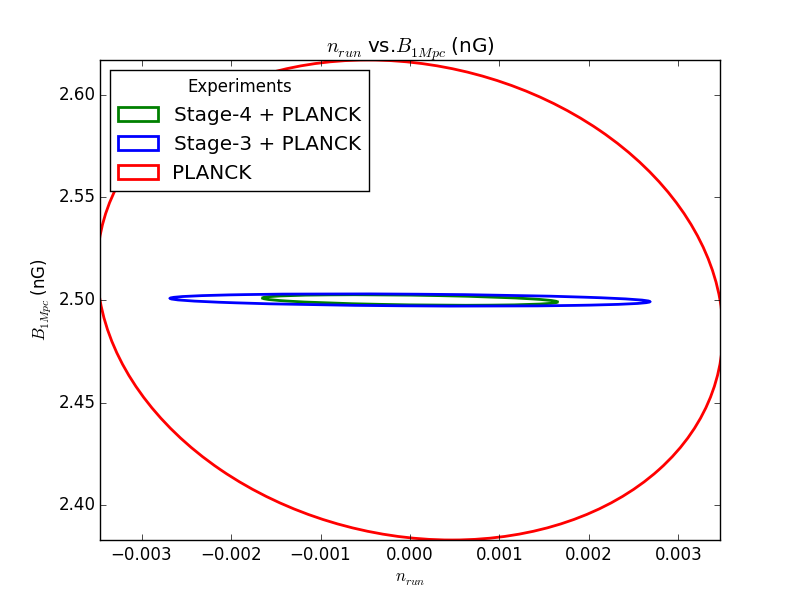
\includegraphics[scale=0.8]{images/contours/nrun.png}
\caption{This is a plot of the 1$\sigma$ confidence contours for $n_{run}$ vs. $B_{1Mpc}$. The red line shows the confidence contour for previous PLANCK data. The blue contour shows the confidence contour for stage-3 CMB experiments plus PLANCK data. The green contour shows the confidence contour for stage-4 CMB experiments plus PLANCK data. The plot shows a large forecasted improvement on the stage-3 and stage-4 precisions on $B_{1Mpc}$ over the previous PLANCK constraints. Improvements on $n_{run}$ increase from PLANCK to stage-3 and again from stage-3 to stage-4.}
\label{fig:nrun}
\end{figure}

\begin{figure}[h]
\centering
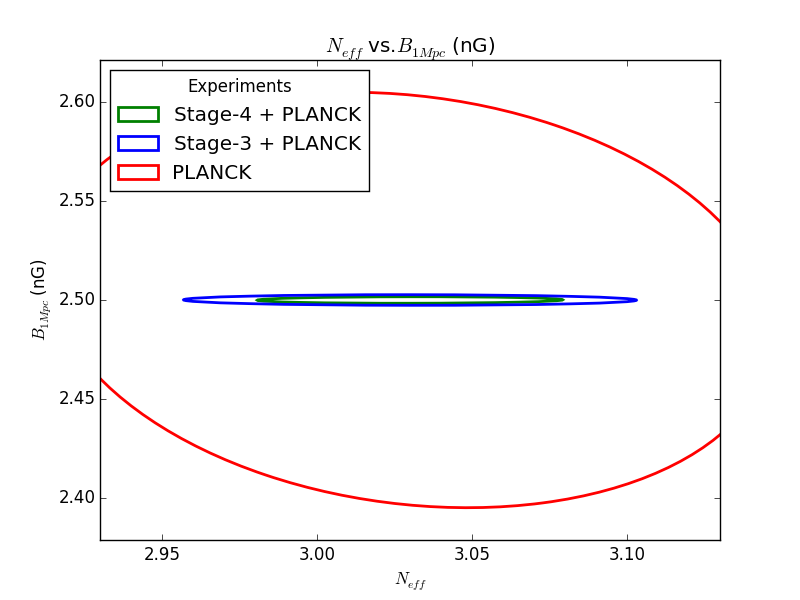
\includegraphics[scale=0.8]{images/contours/neff.png}
\caption{This is a plot of the 1$\sigma$ confidence contours for $N_{eff}$ vs. $B_{1Mpc}$. The red line shows the confidence contour for previous PLANCK data. The blue contour shows the confidence contour for stage-3 CMB experiments plus PLANCK data. The green contour shows the confidence contour for stage-4 CMB experiments plus PLANCK data. The plot shows moderate improvements on $\sigma(B_{1Mpc})$, with stage-4 experiments possessing the tightest constraints, as expected. $N_{eff}$ sees a large forecasted improvement on its constraints from previous PLANCK data. }
\label{fig:neff}
\end{figure}

\begin{figure}[h]
\centering
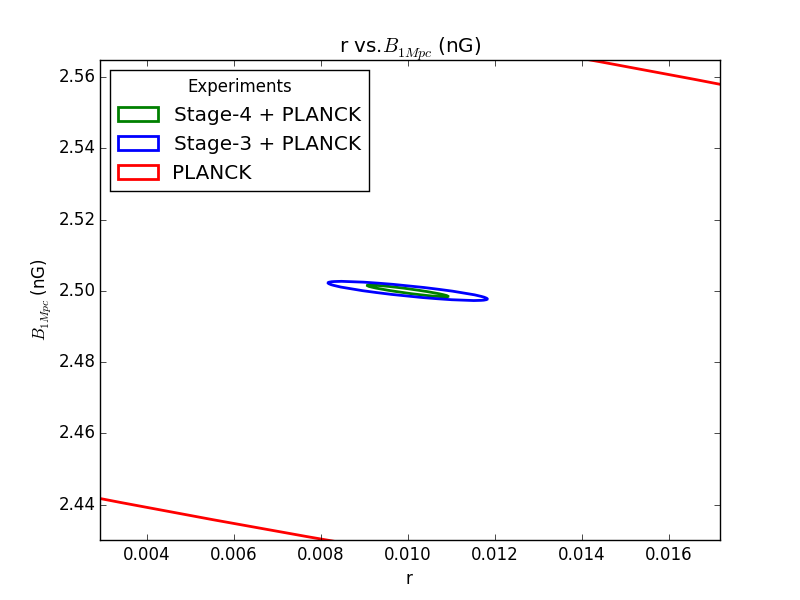
\includegraphics[scale=0.8]{images/contours/52.png}
\caption{This is a plot of the 1$\sigma$ contours for $r$ vs. $B_{1Mpc}$. The red line shows the confidence contour for previous PLANCK data. The blue contour shows the confidence contour for stage-3 CMB experiments plus PLANCK data. The green contour shows the confidence contour for stage-4 CMB experiments plus PLANCK data. There is a large forecasted improvement in both the constraints on $B_{1Mpc}$ and $r$ over previous PLANCK data, however neither stage-3 or stage-4 are expected to break the degeneracy between $B_{1Mpc}$ and $r$.}
\label{fig:r}
\end{figure}
